\documentclass{standalone}
\usepackage{mintikz}

\begin{document}
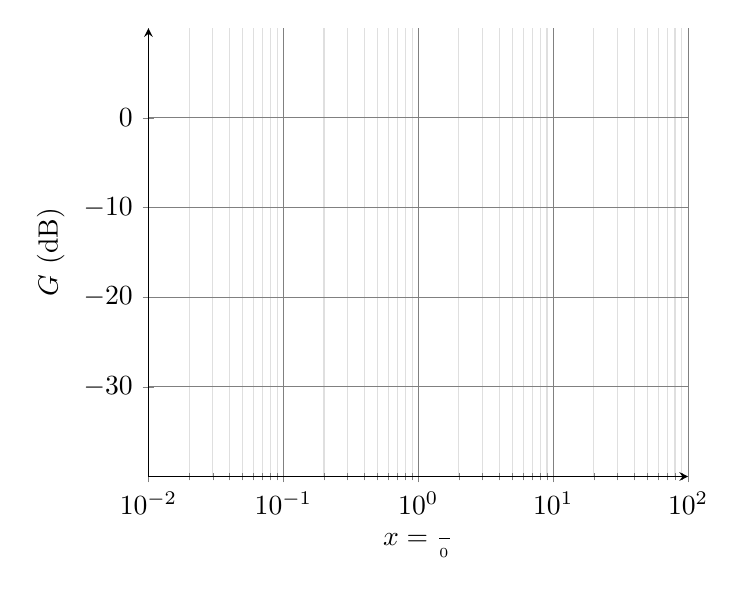
\begin{tikzpicture}[]
	\begin{semilogxaxis}[
			xmin=1e-2, xmax=1e2,
			ymin=-40, ymax=10,
			xlabel={$x=\DS\frac{\w}{\w_0}$}, ylabel=$G_{\dB}$ (dB),
			ytick={-30, -20, ..., 0},
			axis lines=left,
			grid=both,
			major grid style={black!50},
			minor grid style={gray!25},
			clip=true]
		\def\Q{5}
		% \addplot[
		% domain=1e-2:1e2,
		% smooth, thick, red]
		% {-10*log10(1+\Q^2*(\x-1/\x)^2)};
		% \addplot[
		% domain=1e-2:1.3,
		% smooth, black, dashed, thick]
		% {20*log10(\x)-20*log10(\Q)};
		% \addplot[
		% domain=8e-1:1e2,
		% smooth, black, dashed, thick]
		% {-20*log10(\x)-20*log10(\Q)};
		% \def\Q{.5}
		% \addplot[
		% domain=1e-2:1e2,
		% smooth, thick, blue]
		% {-10*log10(1+\Q^2*(\x-1/\x)^2)};
		% \addplot[
		% domain=1e-2:1.3,
		% smooth, black, dashed, thick]
		% {20*log10(\x)-20*log10(\Q)};
		% \addplot[
		% domain=8e-1:1e2,
		% smooth, black, dashed, thick]
		% {-20*log10(\x)-20*log10(\Q)};
		% \node[color=red] at (axis cs:15,5) {$Q=5$};
		% \node[color=blue] at (axis cs:15,0) {$Q=0.5$};
		% \draw[dashed, thick]
		% (axis cs:1e-2,-3) -|
		% (axis cs:1e0,-30);
	\end{semilogxaxis}
\end{tikzpicture}
\end{document}
